\documentclass[10pt,a4paper,twocolumn]{extarticle}
\usepackage[a4paper,margin=1.45cm,columnsep=0.6cm,top=1.3cm,bottom=1.4cm]{geometry}
\usepackage[T1]{fontenc}
\usepackage[utf8]{inputenc}
\usepackage{libertine}
\usepackage[libertine]{newtxmath}
\usepackage{microtype}
\usepackage[scaled=0.82]{beramono}
\usepackage{graphicx}
\usepackage{booktabs}
\usepackage{xcolor}
\usepackage{enumitem}
\usepackage[font=footnotesize,labelfont=bf,skip=3pt]{caption}
\usepackage{titlesec}
\definecolor{accent}{HTML}{2563EB}
\titleformat{\section}{\normalsize\bfseries\color{accent}}{\thesection}{0.5em}{}
\titlespacing*{\section}{0pt}{6pt}{2pt}
\setlist{itemsep=1pt,topsep=2pt,leftmargin=1.1em}
\setlength{\parskip}{2pt}
\setlength{\parindent}{0pt}
\setlength{\textfloatsep}{6pt}
\setlength{\floatsep}{5pt}
\pagestyle{empty}

\begin{document}
\twocolumn[{%
  \begin{center}
    {\Large\bfseries Ignacio Queipo de Llano Pérez-Gascón}\\[2pt]
    {\large Spot-a-hit: deciding which songs to back}\\[1pt]
    {\footnotesize Predictive Machine Learning in Finance · IESE MiF · individual assignment · notebook \texttt{QueipoDeLlano\_Ignacio.ipynb}}
  \end{center}
  \vspace{2pt}
  \hrule
  \vspace{6pt}
}]

\section{The problem is a decision, so the model has to be calibrated}
Backing a hit pays $+1.5$M and backing a flop costs $-0.9$M, so I invest whenever
$P(\text{hit}) > 0.9/2.4 = 0.375$. That means the grade comes from two things at once:
ranking songs well (AUC) and giving probabilities that can be trusted at 0.375 (log-loss).
I tuned everything for log-loss and reported AUC, accuracy and profit, always out of fold on
the 10{,}000 train songs. For reference, investing in everything earns 2{,}602M and perfect
foresight 7{,}251M.

\section{What the data was hiding}
Most of the gain came from reading the data before modelling it.
\begin{itemize}
  \item \textbf{The test titles are masked.} 98.9\% of test titles have asterisks and none
  in train do. Comparing letter frequencies, eleven lowercase letters disappear
  (\texttt{a b c e h i m o s u v} survive 0--5\%, the rest 86--105\%), so the rule is
  deterministic: \emph{Breaking Up Is Hard To Do} $\to$ \emph{Br**k*ng Up I* H*rd T* D*}.
  Applied to train it gives 38.6\% asterisks against 39.0\% in test. I masked the train
  titles the same way, otherwise every title feature would mean one thing in training and
  another in test, and no CV number would have warned me.
  \item \textbf{No test title appears in train}, while 10.7\% of train songs share a title
  (covers, remasters). The split was grouped by title, so my CV is
  \texttt{StratifiedGroupKFold} on the normalised title, also in every inner fold.
  \item \textbf{The artist is almost the label.} 83.5\% of artists with two or more songs
  are pure (all hits or all flops). Splitting credits (\emph{Kid Ink Featuring Chris
  Brown} $\to$ \emph{kid ink}, \emph{chris brown}) raises the share of test songs with a
  known artist from 58\% to 68\%.
  \item The \texttt{id} only encodes the decade (AUC 0.48--0.52 within each decade), so it
  is out.
\end{itemize}

\section{Features}
Two kinds, kept apart on purpose. \textbf{Without the target}, computed on train and test
together (same closed box, no outside data): audio, audio z-scored within its decade, the
artist profile (songs, decades active, mean sound, how far each song is from it), title
shape from the masked text, and audio-kNN neighbours. \textbf{With the target}, always
nested out of fold so no song ever sees its own label: hit and flop counts of the main and
of each credited artist, and a TF-IDF text model with the masked title and the artist in
separate character n-gram spaces (AUC 0.891 alone). 87 features in total.

\section{Models}
\begin{table}[h]
\centering\footnotesize
\begin{tabular}{@{}lccl@{}}
\toprule
Model & AUC alone & corr.\ trees & Role \\
\midrule
LightGBM, CatBoost, XGBoost & 0.947 & -- & backbone \\
Char-level BiGRU & 0.876 & 0.77 & different errors \\
TF-IDF text model & 0.891 & 0.84 & recalibrates text \\
\midrule
\textbf{Stack (logistic)} & \textbf{0.9485} & & \textbf{submitted} \\
\bottomrule
\end{tabular}
\caption{Final pipeline, 10-fold grouped CV.}
\end{table}
\textbf{Gradient boosting.} Three families with Optuna (TPE, log-loss) and three seeds each.
Optuna chose slow learning ($\approx$0.01) and LightGBM column sampling of 0.27: with seven
artist features saying nearly the same thing, forcing each tree to look elsewhere is
regularisation.

\textbf{Char-level BiGRU} on ``masked title $\|$ artist'' (GPU, 96 units, 5 seeds). On its
own it is the weakest model, but its correlation with the trees is only 0.77 and it adds
+0.001 AUC and +32M. A hybrid net that also saw the audio scored much better alone (0.918)
and added nothing, because it learnt what the trees already knew. In an ensemble a weak
model that is wrong in different places is worth more than a good one that agrees.

\textbf{Stack.} Logistic regression on logits of the trees, the BiGRU and the text model,
plus interactions with ``some credited artist is already in train''. It is a clean read:
for a new artist the BiGRU weight is 0.46, for a known one 0.16, because then the artist's
record says more than how the name is spelled. The stack is itself evaluated over
10 folds $\times$ 5 repeats.

\begin{table}[h]
\centering\footnotesize
\begin{tabular}{@{}p{0.47\columnwidth}cp{0.33\columnwidth}@{}}
\toprule
Tried and dropped & AUC & Why \\
\midrule
MLP with entity embeddings & 0.936 & overconfident, corr.\ 0.93 \\
Peer stacking (same-artist guesses) & 0.945 & already in the artist profile \\
Hybrid GRU + audio net & 0.918 & adds 0 in the stack \\
BiGRU nested inside the trees & 0.948 & same as stacking, 2$\times$ slower \\
LightGBM as second level & $\le$0.948 & overfits 3 inputs \\
Pretrained classifier (Jev), no training & 0.918 & knows who was famous: external data \\
\bottomrule
\end{tabular}
\caption{What did not make it into the notebook.}
\end{table}
The last row is worth a line. Out of curiosity I asked a pretrained decision model whether
each of 1{,}000 train songs charted. With audio only it scored 0.68; with the artist's name,
0.918 without seeing a single label. That is memory of the world, exactly what the
assignment forbids and why the titles are masked, so it stays out.

\begin{figure}[t]
\centering
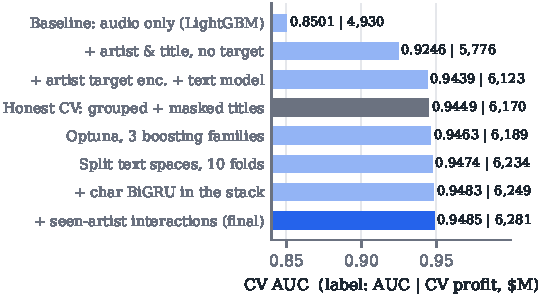
\includegraphics[width=\columnwidth]{fig/progression.pdf}
\caption{How the CV AUC was built. The grey bar is the first honest baseline (grouped CV,
masked train titles); the bars above it are slightly optimistic. Dashed line: 0.95.}
\end{figure}

\section{Results}
\begin{figure}[t]
\centering
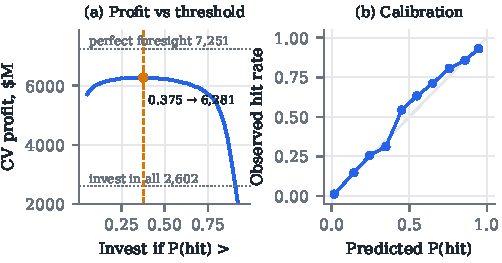
\includegraphics[width=\columnwidth]{fig/profit_calibration.pdf}
\caption{Final model, out of fold. (a) Profit is flat around 0.375, so the theoretical
threshold is also the empirical one. (b) Probabilities sit on the diagonal.}
\end{figure}
Out of fold the final model gets \textbf{AUC 0.9485, accuracy 0.904, log-loss 0.255 and
6{,}281M}, 86.6\% of perfect foresight and 2.4 times investing in everything. The best
empirical threshold is within 5M of 0.375, which is what a calibrated model should give, so
I keep the theoretical one. On test it invests in \textbf{1{,}090 of 2{,}000 songs}. If the
probabilities hold, those 1{,}090 bets carry about 938 hits and an expected profit of
$\sum (2.4\,p - 0.9) \approx 1{,}270$M, in line with the CV figure scaled to 2{,}000 songs
(1{,}256M).

\section{Reproducibility}
The notebook only needs \texttt{train.xlsx} and \texttt{test.xlsx} next to it, writes
\texttt{decisions.csv} and reproduces these numbers to the decimal in 45 minutes
(\texttt{QUICK = True} runs 5 folds and one seed for a fast check, AUC 0.9484). It uses all cores
but two: with \texttt{n\_jobs=-1} LightGBM and CatBoost stalled on my machine.

\section{Conclusion: why 0.9485 is the ceiling}
I did not reach 0.95 in honest CV, and I think three things together say this is the limit
of the data under the rules, not of the ideas.

\textbf{The curve went flat.} From run 10 to 14 five ideas of very different nature (more
folds, a recurrent net, a hybrid net, a nested feature, two kinds of stacker) all land
between 0.947 and 0.9486. A bootstrap of the 10{,}000 out-of-fold predictions gives the final
AUC a standard error of 0.0022, so that whole spread is about half of the noise in a single
estimate. When changes that different stop moving the number, the model is not what is
missing.

\textbf{Capacity is not the bottleneck.} The three boosting libraries score the same to the
fourth decimal (0.9467), a neural net that sees everything scores worse, and the only thing
that still helped was a weak model that was wrong in different places. More model buys
nothing when every model already agrees on what can be learnt.

\textbf{What is left needs outside knowledge.} 15 songs get $P>0.95$ and are labelled
flops, mostly by artists whose other songs of that decade are hits (some look like label
noise). 21 get $P<0.05$ and are hits: a Christmas song by Los del Río, PPAP, a metal cover
of Taylor Swift. They are hits despite how they sound and who sings them. Nothing in the
audio, the masked title or the artist's record separates them, and the three rules of the
assignment close the other doors on purpose: no external data, titles masked so they
cannot be looked up, and a split by title so a cover cannot borrow the original's label.
The Jev test shows the missing piece is exactly that: a model that knows who was famous
reaches 0.918 from names alone, without a single label. The gap from 0.9485 to 0.95 is
music history, and music history is the one thing we are not allowed to bring.

The split by artist says the same: AUC 0.948 for songs whose artist the model has seen and
0.940 for new ones, where only sound and spelling are left. Since 68\% of test songs have a
known artist against 65\% inside the folds, and the final model trains on all of train, I
expect the test to land slightly above the CV, and with 2{,}000 songs the 95\% interval is
wide enough (0.944--0.953 even on 10{,}000) that 0.95 is possible there by luck. I would
rather explain 0.9485 than defend a number I don't believe.

\end{document}
